\chapter{Exercise 07}
\extitle{Polynomial models}
%******************************************************************************%
%                                                                              %
%                                 Interlude                                    %
%                         for Machine Learning module                          %
%                                                                              %
%******************************************************************************%

% =============================================== %
\section*{Interlude - Introducing Polynomial Models}
% ----------------------------------------------- %

You probably noticed that the method we use is called \textit{linear regression} for a reason:
the model generates all of its predictions on a straight line.
However, we often encounter features that do not have a linear relationship with the predicted variable,
like in the figure below:

\begin{figure}[!h]
    \centering
    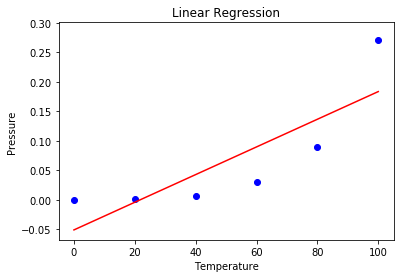
\includegraphics[scale=0.6]{assets/polynomial_straight_line.png}
    \caption{Non-linear relationship}
\end{figure}

In that case, we are stuck with a straight line that cannot fit the data points properly.
In this example, what if we could express $y$ not as a function of $x$, but also of $x^2$, and maybe even $x^3$ and $x^4$?
We could make a hypothesis that draws a nice \textbf{curve} that would better fit the data.
That's where polynomial features can help!

% =============================================== %
\section*{Interlude - Polynomial features}
% ----------------------------------------------- %
First we get to do some \textit{feature engineering}.
We create new features by raising our initial $x$ feature to the power of 2, and then 3, 4... as far as we want to go.
For each new feature we need to create a new column in the dataset.

% =============================================== %
\section*{Interlude - Polynomial Hypothesis}
% ----------------------------------------------- %
Now that we created our new features, we can combine them in a linear hypothesis that looks just the same as what we're used to:

$$
\hat{y} = \theta_0 + \theta_1 x  +\theta_2 x^{2} + \dots + \theta_n x^{n}
$$  

It's a little strange because we are building a linear combination, not with different features but with different powers of the same feature.
This is a first way of introducing non-linearity in a regression model!
\newpage
\turnindir{ex07}
\exnumber{07}
\exfiles{polynomial\_model.py}
\exforbidden{sklearn}
\makeheaderfilesforbidden


% ================================= %
\section*{Objective}
% --------------------------------- %
Broaden your comprehension of the concept of hypothesis.\\
\newline
Create a function that takes a vector $x$ of dimension $m$ and an integer $n$ as input, and returns a matrix of dimensions $(m \times n)$.
Each column of the matrix contains $x$ raised to the power of $j$, for $j = 1, 2, ..., n$:

$$
\begin{matrix}
x &|& x^2 &|& x^3 &|& \ldots &|& x^n
\end{matrix}
$$
Such a matrix is called a \textbf{Vandermonde matrix}.

% ================================= %
\section*{Instructions}
% --------------------------------- %
In the \texttt{polynomial\_model.py} file, create the following function as per the instructions given below:\\
\\
\begin{minted}[bgcolor=darcula-back,formatcom=\color{lightgrey},fontsize=\scriptsize]{python}
def add_polynomial_features(x, power):
    """Add polynomial features to vector x by raising its values up to the power given in argument.  
    Args:
      x: has to be an numpy.array, a vector of dimension m * 1.
      power: has to be an int, the power up to which the components of vector x are going to be raised.
    Return:
      The matrix of polynomial features as a numpy.array, of dimension m * n,
        containing the polynomial feature values for all training examples.
      None if x is an empty numpy.array.
      None if x or power is not of expected type.
    Raises:
      This function should not raise any Exception.
    """
    ... Your code ...
\end{minted}

% ================================= %
\section*{Examples}
% --------------------------------- %
\begin{minted}[bgcolor=darcula-back,formatcom=\color{lightgrey},fontsize=\scriptsize]{python}
import numpy as np
x = np.arange(1,6).reshape(-1, 1)


# Example 0:
add_polynomial_features(x, 3)
# Output:
array([[  1,   1,   1],
       [  2,   4,   8],
       [  3,   9,  27],
       [  4,  16,  64],
       [  5,  25, 125]])


# Example 1:
add_polynomial_features(x, 6)
# Output:
array([[    1,     1,     1,     1,     1,     1],
       [    2,     4,     8,    16,    32,    64],
       [    3,     9,    27,    81,   243,   729],
       [    4,    16,    64,   256,  1024,  4096],
       [    5,    25,   125,   625,  3125, 15625]])
\end{minted}